\chapter{The RMT 2.0}
\label{results}
\textcolor{red}{1 - RMT 2.0\\
2 - Testes com projetos\\
3 - Comparação da RMT 1 com 2
}

\section{The Renewed Cloud Based Architecture}
\label{sec-cloud}
The revised architecture introduces several modifications to the communication protocols between services. The initial version of the tool had three services and one Java desktop application. The revised architecture transitioned the desktop application to a web-based platform, altering each service's operational dynamics. The newly devised architecture is illustrated in \Cref{fig-architecture}.

\begin{figure}[ht!]
\SetCaptionWidth{\textwidth}
\caption{RMT revised architecture diagram}
\label{fig-async}
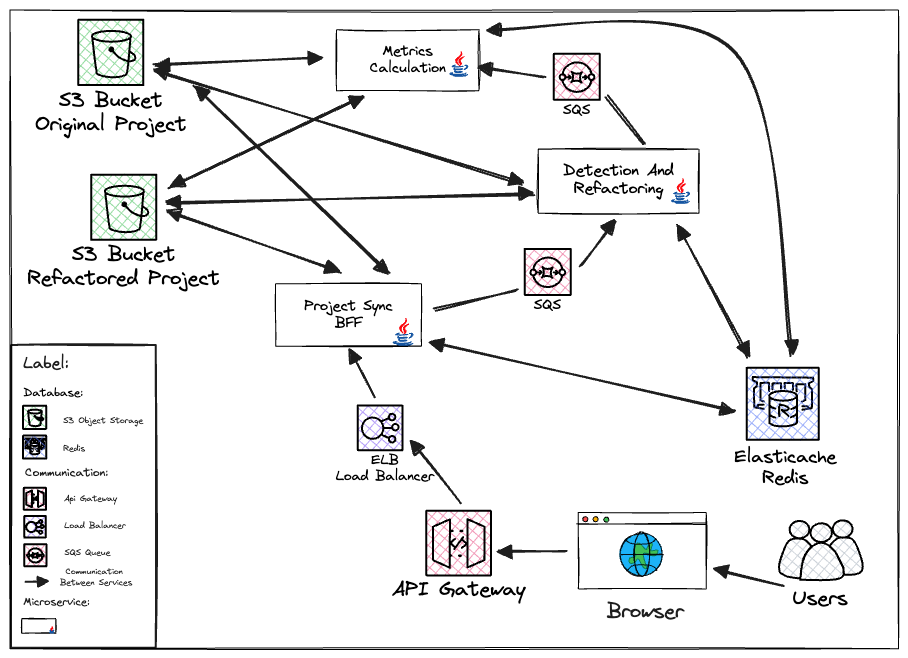
\includegraphics[width =\textwidth, scale=0.2]{Chapter-5/Figures/Async.png}
\SourceOrNote{Own authorship (2024)}
\end{figure}
\FloatBarrier

\subsection{Comunication Improvements}

The communication type was switched to queues instead of HTTP requests. The modification primarily aims to establish a communication mechanism with enhanced configurability in the event of failures, as the services must acknowledge the messages, or they will be retried as often as configured. Queues also offer an asynchronous communication that is out of the box. Otherwise, in the HTTP request, the retry has to be implemented on the client side according to the server response. It is also possible to have an HTTP asynchronous request, but it must be implemented on the client side.

The Simple Queue Service (SQS) operates in its default configuration, implementing a quintuple retry mechanism to transmit a JSON object containing the project identifier between microservices.

\subsection{Storage \& Database Improvements}

The initial version of RMT utilizes MongoDB GridFs for file storage, a feature designed to facilitate the preservation of files within the database architecture. The updated version uses Amazon S3 for project storage, using a dual-bucket strategy: one designated for the original project and the other for the refactored iterations. All microservices are granted access to the designated buckets, enabling seamless file storage and retrieval. The project information and statuses are stored in the Redis in-memory document database, and all services have access.

\section{RMT 2.0 Package Arrangement}

\begin{figure}[ht!]
\SetCaptionWidth{\textwidth}
\caption{Project Sync BFF package diagram}
\label{fig-project-sync-package}
\fontsize{8}{10}\selectfont
\includesvg[width =\textwidth]{Chapter-5/Figures/project-sync-bff.svg}
\SourceOrNote{Own authorship (2024)}
\end{figure}
\FloatBarrier


\begin{figure}[ht!]
\SetCaptionWidth{\textwidth}
\caption{Detection and Refactoring service package diagram}
\label{fig-detection-refactoring-package}
\includesvg[width =\textwidth]{Chapter-5/Figures/detection-and-refactoring.svg}
\SourceOrNote{Own authorship (2024)}
\end{figure}
\FloatBarrier

\begin{figure}[ht!]
\SetCaptionWidth{\textwidth}
\caption{Metrics Calculator service package diagram}
\label{fig-metrics-calculator-package}
\includesvg[width =\textwidth]{Chapter-5/Figures/metrics-calculator.svg}
\SourceOrNote{Own authorship (2024)}
\end{figure}
\FloatBarrier



\section{Services Behavior Improviments}
\label{sub-services-behaivour}

Notwithstanding recent updates to the tool, its resultant behavior remains unchanged. The tool now runs with a linear execution flow, obviating the need for interservice communication during project refactoring. Given the process's asynchronous nature, users must request the completion status to display the retrieved relevant information. The process is represented in \cref{fig-activity-diagram}, with the blue nodes representing the behavior inherited from the initial version of the tool.

\begin{figure}[ht!]
\SetCaptionWidth{\textwidth}
\caption{RMT 2.0 Activity Diagram}
\label{fig-activity-diagram}
\fontsize{5.8}{8}\selectfont
\includesvg[width =\textwidth]{Chapter-5/Figures/activity-refactored-rmt.svg}
\SourceOrNote{Own authorship (2024)}
\end{figure}
\FloatBarrier

The flow starts with the user selecting the project and sending it to the API Gateway connected to the Project Sync BFF; the service sends the project ID to the refactoring queue to start the process. The Detection and Refacred Service will immediately search for the candidates to be refactored and apply the refactoring. A message with the project ID is sent to the metrics calculation queue if any candidate is found. The Metrics Calculation Service computes the quality attributes for the project and ends the processing. The Project Sync BFF service offers a pull mechanism that consults Redis looking for a final status and, if found, returns the project information and metrics. The behavior is displayed in \Cref{fig-activity-diagram}.

\section{Testing RMT 2.0}
\label{sub-tests}

\subsection{Testing Through Refactored Article Application Exemplars}

The implementations exemplified by \textcite{liu2014automated} and \textcite{zafeiris2017automated} were used for the preliminary evaluation.

To refactor using the factory method design pattern, \textcite{liu2014automated} introduces four distinct classes: a \texttt{Logger} interface, 	\texttt{FileLogger} and \texttt{DatabaseLogger} which implement the interface, and the \texttt{LoggerFactory} serving as a factory to select among the implementations. The \cref{fig-factory-client} displays the refactored \texttt{LoggerFactory} that was changed to abstract; the implementation was moved to the \texttt{FileLoggerFactory} and \texttt{DatabaseLoggerFactory}. The metrics displayed are positive, indicating an improvement in maintainability and reusability without changing reliability.

\begin{figure}[ht!]
\SetCaptionWidth{\textwidth}
\caption{Refactored Project For Factory Method}
\label{fig-factory-client}
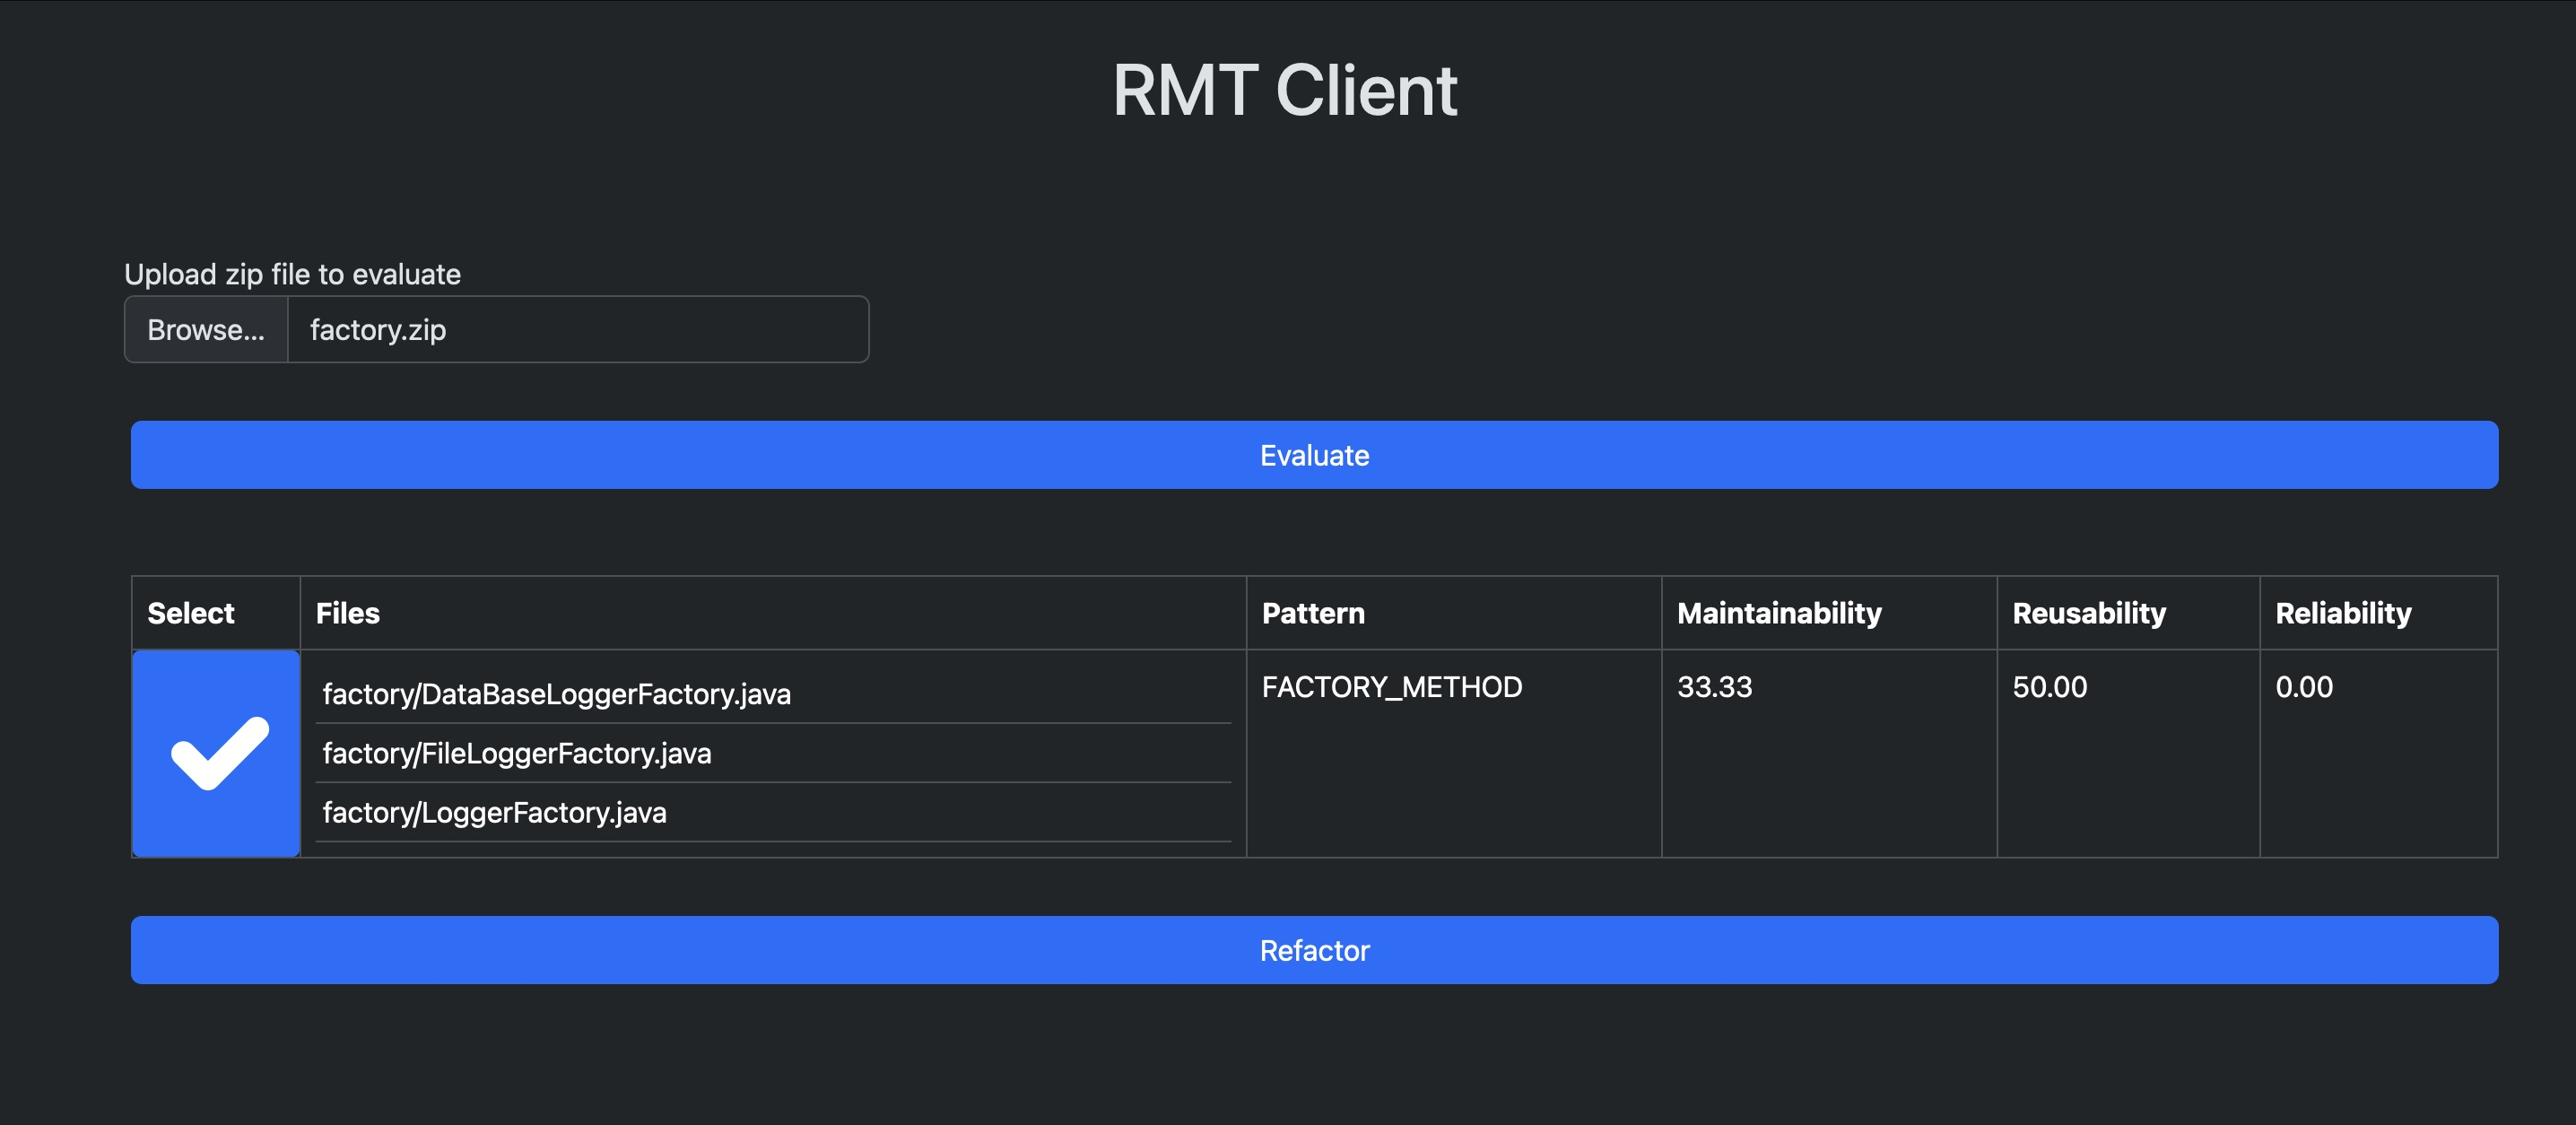
\includegraphics[width =\textwidth]{Chapter-5/Figures/rmt-factory-client.jpeg}
\SourceOrNote{Own authorship (2024)}
\end{figure}
\FloatBarrier

To exemplify the strategy pattern \textcite{liu2014automated}, create the \texttt{MovieTicket} class, which has an if statement for each ticket type. The method creates an abstract \texttt{Strategy} class with the calculate method, the code extracted from the \texttt{MovieTicket} is implemented on the \texttt{ConcreteStrategyS}, \texttt{ConcreateStrategyM} and \texttt{ConcreateStrategyC}. The maintenance and reusability metrics improved, although reliability decreased, as shown in \cref{fig-strategy-client}.

\begin{figure}[ht!]
\label{fig-strategy-client}
\caption{Refactored Project For Strategy}
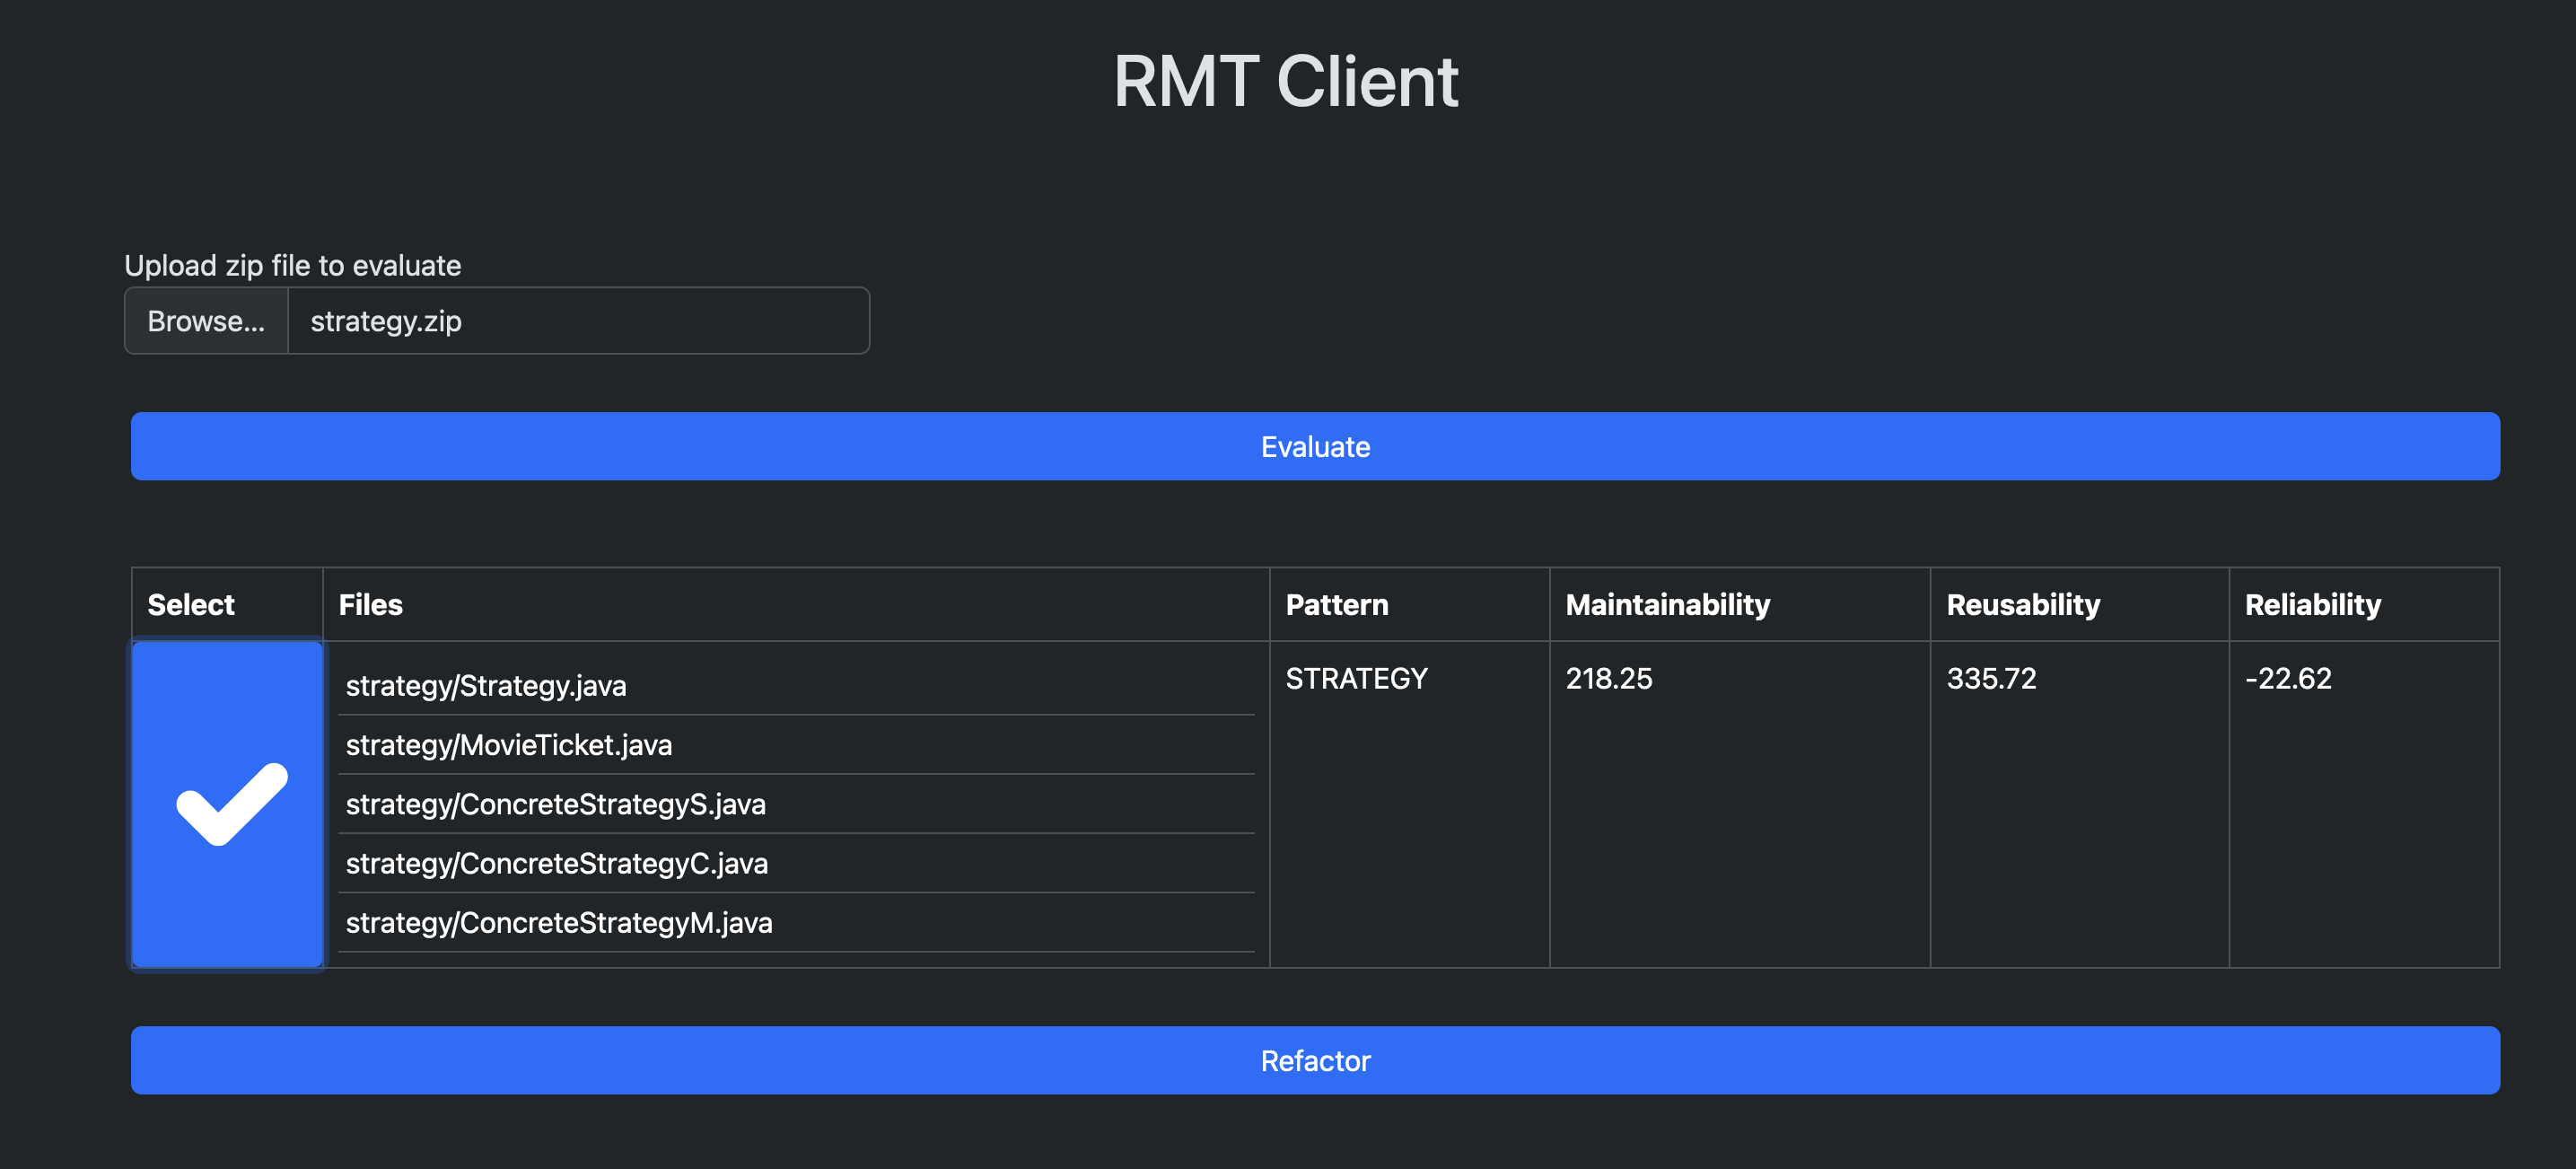
\includegraphics[width =\textwidth]{Chapter-5/Figures/rmt-strategy-client.png}
\SourceOrNote{Own authorship (2024)}
\end{figure}
\FloatBarrier

The \textcite{zafeiris2017automated} implements the template method using the jade-test-suit to exemplify the process. The \texttt{JICPPeer} class is the parent of the \texttt{JICPSPeer} class, which implements a method that has a \texttt{super} call; the refactoring extract code before and after the super call into new methods and replaces the super call to a method call with the same behavior. The maintainability, reusability, and reliability metrics are negative, showing a deterioration. It is represented in \cref{fig-template-client}

\begin{figure}[ht!]
\label{fig-template-client}
\caption{Refactored Project For Template Method}
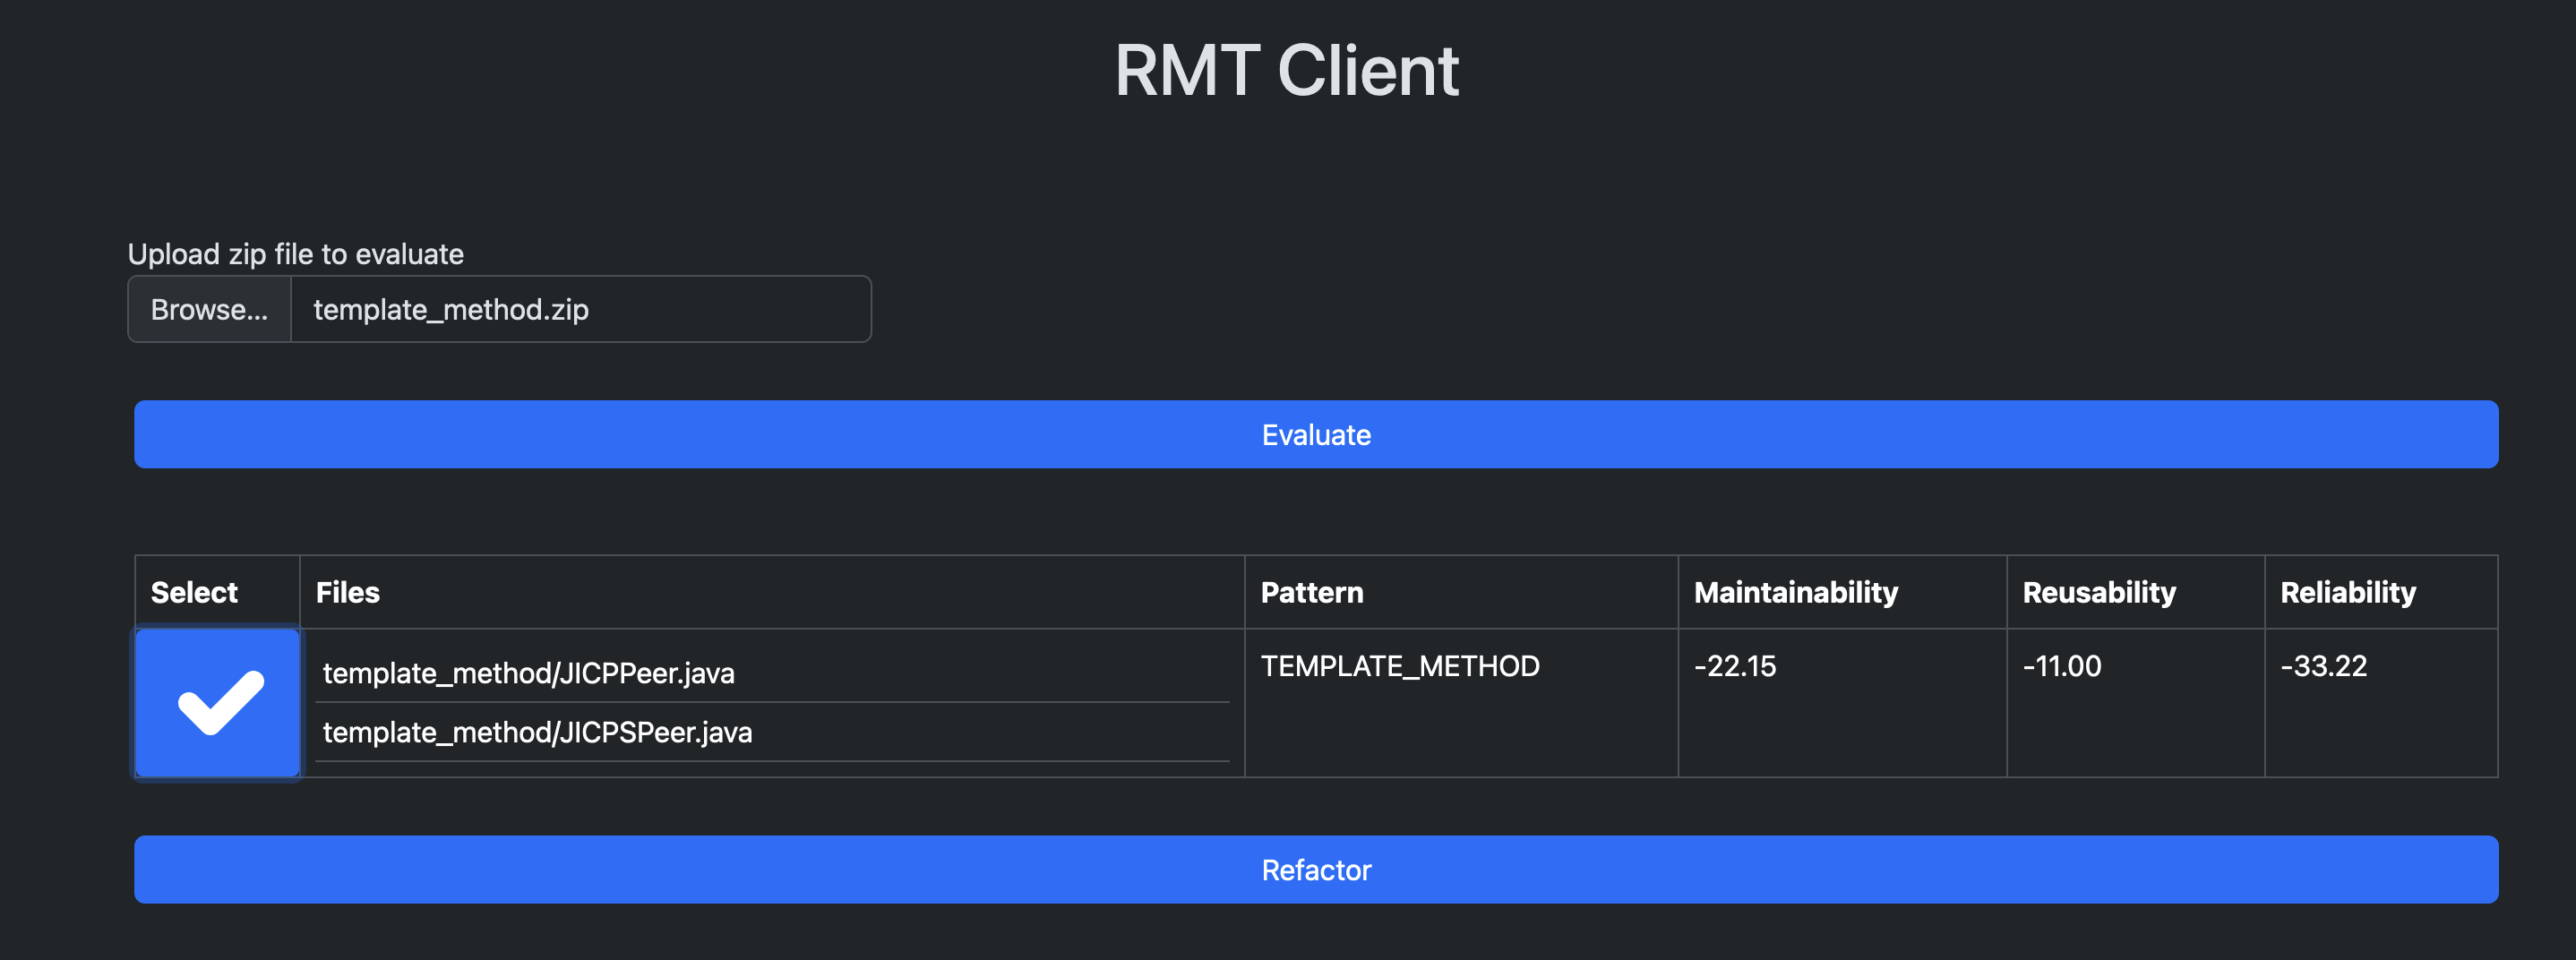
\includegraphics[width =\textwidth]{Chapter-5/Figures/rmt-template-client.png}
\SourceOrNote{Own authorship (2024)}
\end{figure}
\FloatBarrier

An additional approach to test the tool and ensure its quality will undergo a self-scanning procedure. The analysis was performed to test the effectiveness of the tool, with a focus on evaluating RMT and its next version, RMT 2.0. Examining both RMT versions showed that there were no elements that needed refactoring. 

\section{Comparing RMT versions}

\section{Closing Remarks}
\label{sec-closingproposal}
